\documentclass{article}
\title{\textbf{R Lab One}}
\author{\textbf{Katherine Wolf}\\ Introduction to Causal Inference (PH252D)\\ \today}
\date{}

% list of latex packages you'll need
\usepackage{float}  % for tables
\usepackage{mathtools}  % for mathematical symbols
\usepackage{bm}  % to bold mathematical symbols like betas
\usepackage{scrextend}  % to indent subsections
\usepackage{xltxtra}
\usepackage{fontspec}
\usepackage{xunicode}
\usepackage[dvipsnames]{xcolor}
\usepackage{soul}  % get underlines
\usepackage[skip=0.5\baselineskip]{caption}  % control caption printing space
\usepackage{longtable}
\usepackage{amsmath}
\usepackage{amsfonts}
\usepackage{bm}
\usepackage{caption}
\usepackage[shortlabels]{enumitem}

% set fonts
\setmainfont{Georgia}
\setsansfont[Scale=MatchLowercase]{Arial}  % sets the sans font
\setmonofont[Scale=MatchLowercase]{inconsolata}  % sets the monospace font

% make special code formatting
\NewDocumentCommand{\codeword}{v}{%
  \texttt{\textcolor{RoyalPurple}{#1}}%
}

% set the margins of the document
\usepackage[top=1in, bottom=1in, left=.5in, right=.5in]{geometry}
\setlength\parindent{0pt}

% end the preamble and begin the document
\begin{document}

\maketitle

\vspace{2mm}

\textbf{\textit{Step 1: State the scientific question.}}

\begin{enumerate}[label=\textbf{(\alph*)}]

  \item \textbf{What causal question or questions was this research aiming to answer?}
  
  What is the effect of circumcision on cumulative HIV incidence after two years?  (Stated more counterfactually: How would cumulative HIV incidence have differed after two years if everyone in the target population were circumcised at or before baseline versus if no one in the target population were circumcised at baseline?)
  
  \item \textbf{What makes this a causal question as opposed to a purely statistical question?}
  
  This question is a causal question because it asks how the distribution of the outcome, HIV incidence at two years, would change if the distribution of the exposure, circumcision at baseline, changed in the target population, whereas a statistical question asks how the distribution of the outcome is associated with the distribution of the exposure in the target population as is.
  
  \textbf{Give an example of a purely statistical question that the research described could address.}

  How did the risk of HIV at two years after baseline in the target population differ between participants who were circumcised at baseline and those who were not?

  \textbf{Is the language used by the authors in describing their objective causal or statistical?}
  
  The language in the title of the study, "The protective effect of circumcision on HIV incidence in rural low-risk men circumcised predominantly by traditional circumcisers in Kenya: two-year follow-up of the Kericho HIV Cohort Study," implies causality, as it talks about an "effect" of circumcision "on" HIV incidence, implying that the authors believe that circumcision affected HIV incidence in some way. 
  
  In the study abstract, however, the authors' language is statistical ("we examined the association between circumcision and HIV infection in a cohort of adult agricultural workers and dependents after two years of follow-up"), as they state that they examined the observed association as-is, and do not elsewhere claim that they attempted to isolate the effect of circumcision on HIV incidence were the intervention of circumcision manipulated in the same underlying population.
  
  \item \textbf{Specify the target population.}
  
  The target population was adult agricultural workers (presumably limited to men with penises) their and dependents in rural Kenya.

\end{enumerate}

\pagebreak

\textbf{\textit{Step 2: Specify a structural causal model (SCM).}}

\vspace{2mm}

\textbf{Use the formal notation defined in class. Recall that $\bm{W}$ denotes baseline (pre-exposure) covariates, $\bm{A}$ the exposure or treatment, and $\bm{Y}$ the outcome. Feel free to split your covariates into $\bm{W_1, W_2, ...}$ as needed, but please define your random variables. If needed, use $\bm{Z}$ to denote a random variable, occurring after the exposure but before the outcome.}

\vspace{2mm}

\textbf{The data collected should give you some idea of the covariates that could be included, but there may be additional ones. When needed, we have attempted to provide additional background material to facilitate model specification. You and your group should be able to fill in the remaining material. However, do not be too concerned if you are unsure of some of the relationships in your model.}

\begin{enumerate}[label=\textbf{(\alph*)}]

  \item \textbf{What are the endogenous variables $\bm{X}$? What additional covariates besides those observed might be important? How would you incorporate them into the model?}
  
  The endogenous variables $\bm{X}$ include $\bm{X} = \{\bm{W} = \{W_1, \dots, W_i \}, \bm{Z} = \{Z_1, \dots, Z_j \}, A, Y\}$, where
  \begin{itemize}
    \item $\bm{W}$ is a vector of random variables representing the pre-exposure baseline covariates affecting the exposure of circumcision by baseline, which here might be
    \begin{itemize}
      \item $W_1$: tribe at baseline,
      \item $W_2$: religion at baseline,
      \item $W_3$: self-reported sex with a commercial sex worker at baseline, and
      \item $W_4$: self-reported diagnosis with a sexually transmitted infection at baseline;
    \end{itemize}
    \item $\bm{Z}$ is a vector of random variables representing covariates occurring after and affected by the exposure, circumcision status at baseline, that might also affect the outcome. Here an example might be, for example, changes in sexual activity during the study due to circumcision status, for example,
    \begin{itemize}
      \item $Z_1$: decreased condom usage during the study period due to perceived lowered HIV transmission usage post-circumcision in circumcised participants,
      \item $Z_2$: decreased sexual activity during the study period due to decreased sexual pleasure post-circumcision;
    \end{itemize}
    \item $\bm{A}$ is a random variable representing the exposure, here, self-reported circumcision at baseline; and
    \item $\bm{Y}$ is a random variable representing the outcome, here, HIV status at two years of follow-up.
  \end{itemize}
  
  The endogenous variables $\bm{X}$ are those, whether observed or unobserved, that we presume both are affected by and affect other variables in the model. Another endogenous variable or covariate that might be important, for example, is cumulative immune system burden, which, for example, could be affected by a diagnosis with a sexually transmitted infection and also affect the probability of the outcome, HIV incidence. We would incorporate it into the model by making it another $W_i$ variable, even if we didn't measure it.  Age, for example, might also be another important covariate, and could similarly become another $W_i$ variable.
  
  \item \textbf{Discuss your exogenous variables $\bm{U}$. What factors might be included? Did you observe your $\bm{U}$? Could you observe your $\bm{U}$?}
  
  Exogenous variables $\bm{U}$ include all the unobserved variables that are not affected by other factors in the model but go into determining the values of the endogenous $\bm{X}$ variables. For example, $U_{W_1}$ is a random variable representing the unobserved influences on the endogenous variable $W_1$, here specified to represent the participant tribe. The joint distribution of the exogenous variables is represented by the symbol $\bm{P_U}$, i.e., $\bm{U_X} = \{\bm{U_W}, U_A, \bm{U_Z}, U_Y\} \sim \bm{P_U}$. We did not observe the exogenous variables $\bm{U}$ in the current study because exogenous variables are not observed in the current study by definition. Observing them might be possible in other circumstances, though, particularly as science advances. If we do observe a variable in $\bm{U}$, it then becomes one of the variables in $\bm{X}$.
  
  \item \textbf{Specify your structural equations $\bm{F}$. (Please be mindful of the notation used in class.) Do your structural equations make any assumptions about functional form?}
  
  The structural equations are

  \begin{itemize}
  
    \item $\bm{W} = f_{\bm{W}} (\bm{U_W})$
    \item $A = f_{A}(\bm{W}, U_{A})$
    \item $\bm{Z} = f_{\bm{Z}}(A, \bm{W}, \bm{U_Z})$
    \item $Y = f_Y(A, \bm{W}, \bm{Z}, U_Y)$
  
  \end{itemize}

  These equations do not make assumptions about the functional form of any of the causal relationships, as the $f$ terms mean "function of" without specifying the form of each function, although they do list the random variables presumed to determine the ultimate value of each function.
 
  \item \textbf{Discuss any exclusion restrictions. In general, what are exclusion restrictions? What do they mean in words?}
  
  Exclusion restrictions are restrictions on the parents of a random variable in the set $\bm{X}$, in which the omissions of variables in the parent set of a random variable in $\bm{X}$ represent assumptions that the omitted variables do not directly affect that variable.  
  
  \textbf{For the study, do you feel that any are justified?}
  
  I have built the model above to be a recursive (acyclic) structural causal model, meaning that I have assumed that an ordering exists such that each $\bm{X_K}$ in $\bm{X}$ is a function of a subset of its predecessors. Thus 
  \begin{itemize}
      \item $\bm{W}$ excludes $A$, $\bm{Z}$, and $Y$ from its parent set,
      \item $A$ excludes $\bm{Z}$ and $Y$ from its parent set, and
      \item $\bm{Z}$ excludes $Y$ from its parent set.
  \end{itemize} 
  
  Thus I presume here that 
  \begin{itemize}
      \item the variables in $\bm{W}$ (here, tribe and religion) are not affected by circumcision status at baseline $A$, sexual behaviors after circumcision during the study period in $\bm{Z}$, or HIV incidence at the end of the study period $Y$;
      \item circumcision status at baseline $A$ is not affected by sexual behaviors after circumcision during the study period $\bm{Z}$ or HIV incidence at the end of the study period $Y$; and
      \item sexual behaviors after circumcision during the study period $\bm{Z}$ are not affected by HIV incidence at the end of the study period $Y$.
  \end{itemize}
  
  Although I can conceive of scenarios where such restrictions do not hold (for example, an individual changing religious affiliations over anger at involuntary infant circumcision or in response to particular sexual experiences), most of them seem reasonable:
    \begin{itemize}
      \item Given that HIV is asymptomatic in its early stages and that participants only learn their HIV status at the end of the study if they don't have symptoms, excluding HIV incidence from the parent sets of the other variables in $\bm{X}$ before the end of the study seems justified;
      \item Given that the sexual behaviors after circumcision $\bm{Z}$ happen by definition during the study and after the exposure of circumcision status at baseline $A$ or the other covariates collected at baseline $\bm{W}$, those behaviors cannot affect covariates recorded before them in time, so excluding them from the parent sets of $A$ and $\bm{W}$ seems justified; and
      \item Circumcision status at baseline $A$ might or might not affect the values of the covariates in $\bm{W}$, so the assumption that circumcision status at baseline $A$ is not in the parent sets of the variables tribe $W_1$, religion $W_2$, self-reported sex with a commercial sex worker $W_3$, or self-reported diagnosis with a sexually transmitted infection $W_4$, all at baseline, is perhaps the least justified.  \textcolor{red}{COME BACK HERE}
  \end{itemize}
  
  
  
  \item \textbf{Discuss any independence assumptions. In general, what are independence assumptions? What do they mean in words? For the study, do you feel that any are justified? When might they be?}
  
  \item \textbf{Draw at least one possible causal graph.}
  
\end{enumerate}

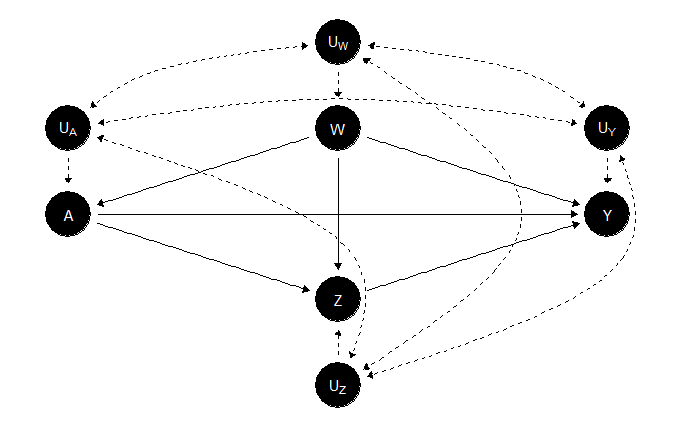
\includegraphics[scale=1]{dag_one.png}


\pagebreak





\textbf{\textit{Step 3: Define the target causal parameter.}}

\vspace{2mm}

\textbf{Carefully consider the causal question or questions this research was aiming to answer.}

\begin{enumerate}[label=\textbf{(\alph*)}]

  \item \textbf{Specify the intervention node(s).}
  
  The intervention node is $A$, an indicator variable for circumcision at baseline.

  \item \textbf{Specify the intervention(s) of interest.}
  
  The intervention of interest is circumcision at the start of the study.

  \item \textbf{Formally express this modification of experimental conditions as an intervention on the SCM and on the causal graph.}
  
  Intervention on the structural causal model:
  
  \begin{itemize}
  
    \item $\bm{W} = f_{\bm{W}} (\bm{U_W})$
    \item $A = a$
    \item $\bm{Z} = f_{\bm{Z}}(A = a, \bm{W}, \bm{U_Z})$
    \item $Y = f_Y(A = a, \bm{W}, \bm{Z}, U_Y)$
  
  \end{itemize}
  
  
  Intervention on the causal graph:
  
  \vspace{2mm}
  
  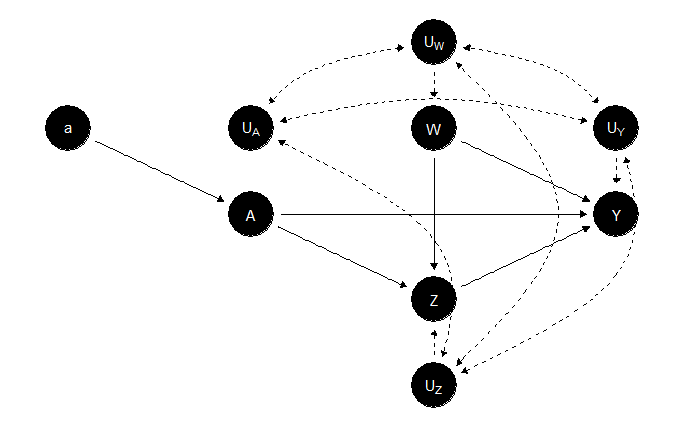
\includegraphics[scale=0.8]{dag_two.png}

  \item \textbf{Specify your counterfactual outcomes under the intervention(s) of interest. How are these counterfactuals defined with an SCM? What do they mean (in words)?}
  \begin{itemize}
  \item $Y_1$: HIV incidence after two years under intervention of circumcision at baseline, $a = 1$.
  \item $Y_0$: HIV incidence after two years under intervention of no circumcision at baseline, $a = 0$.
  \end{itemize}

  Formally, $Y_a = f_{Y}(\bm{W}, a, \bm{Z}, U_{Y}), a \in A = \{0, 1\}.$

  \item \textbf{Using counterfactual notation, define a target causal parameter without using a marginal structural model. What does it mean (in words)?}

  A target causal parameter might be the causal risk difference,

  $E_{U, X}[Y_1]$ - $E_{U, X}[Y_0]$,

  which is the difference in the risk of incident HIV within two years if the whole population had been circumcised at baseline versus if the entire population had been uncircumcised at baseline. 

  \item \textbf{\textit{Bonus:} Using counterfactual notation, define a target causal parameter using a working marginal structural model (MSM). What does it mean (in words)?}

  $E_{U, X}(Y_a) = m(a|\bm{\beta}) = expit(\beta_0 + \beta_1 a)$

  This models the risk of HIV incidence using a logistic model, in which the log odds of HIV incidence equals a linear combination of the baseline log odds of HIV incidence $\beta_0$ plus an indicator variable $a$ for circumcision status times a coefficient $\beta_1$ for the log odds ratio comparing the odds of incident HIV in circumcised men in the numerator to the odds of incident HIV in uncircumcised men in the denominator.
  
\end{enumerate}

\pagebreak

\textbf{\textit{Comments and Additional Questions.}}

\vspace{2mm}

\textbf{Think through the following additional questions and be ready to present your answers in class.}

\begin{itemize}

  \item \textbf{When specifying your SCM, you do not need to incorporate loss to follow up, death, or potential reporting bias. We will learn how to incorporate these later in the course.}

  \item \textbf{When using a marginal structural model to define the target parameter, feel free to refine your research question. However, be able to explain why the modified question is interesting.}
  
\end{itemize}

\begin{enumerate}[label=\textbf{(\alph*)}]

  \item \textbf{How would you formally incorporate the following information in your causal model: in this population men did not alter their sexual behavior because of their circumcision status?}

  I would use an exclusion restriction to eliminate circumcision status $A$ as a potential parent of the covariates in $\bm{Z}$ related to sexual behavior and include them instead in the vector of covariates not in the causal pathway, $\bm{W}$ (i.e., eliminate $A$ from the structural equations for the elements of $\bm{Z}$ related to sexual behavior and add those elements to $\bm{W}$, or, in the diagram, eliminate the edges from $A$ to those elements of $\bm{Z}$ and instead put them in $\bm{W}$).

\vspace{2mm}

  \textbf{Do you think  such  an  assumption  is  warranted  here?}   
  
  No. We don’t have any information here to support such an assumption. Circumcision might alter the experience of and desire for sex with or without a condom, for example, or people might select sex partners with penises in part based on their circumcision statuses.

\vspace{2mm}

  \textbf{Would  it  be  warranted  if  there  were  a  program implementing adult male circumcision as an HIV prevention strategy?} 

  No. Men circumcised through the program, for example, might perceive the treatment as protective against HIV transmission and alter their sexual behaviors as a result, or potential sex partners might select for men circumcised in the program and reject those who had not participated, or vice versa.

\vspace{2mm}

  \textbf{If you are not sure, how would you incorporate this uncertainty in your model?}
    
  If I were unsure, though, I would leave circumcision status $A$ as a potential parent of the elements of the $\bm{Z}$ covariates related to sexual behavior at this step of the model-building.

  \item \textbf{What makes the Kericho population a potentially interesting system to study (as compared, for example, to a population enrolled in a randomized trial)? What might make it less interesting or relevant than other populations? (Think about how you are hoping to use the results of this analysis.)}
  
  The Kericho population might be interesting to study because results from the Kericho population might be more generalizable to other rural populations in Kenya than the randomized trial results, as a randomized trial of circumcision would require all those entering the trial to have uncircumcised penises at baseline and be willing to undergo circumcision. Those trial entry requirements might limit generalizability to populations without those characteristics, as the joint distribution of covariates affecting the exposure of circumcision and the outcome of HIV incidence might differ widely between the population meeting the criterial for entry into the trial and general rural populations in Kenya and similar countries.  In other words, studying the Kericho population might provide additional information on the potential population-level effects of a circumcision intervention on the prevention of HIV incidence on tea plantation workers Kericho and potentially in other workers in other rural areas in Kenya.

  That said, results from the Kericho population might be less useful or relevant if we could not measure the covariates that affect both circumcision and HIV incidence in this population, as unmeasured confounding might limit our ability to infer causality in the population.

\end{enumerate}


\pagebreak


Equation:

$$ \log(h(t|\mathbf{x}, \bm{\beta})) =  \log[h_0(t)] + \beta_1\mathbb{I}(x_1 = 1) + \beta_2 x_2 + \beta_3\mathbb{I}(x_3 = 1) + \beta_4\mathbb{I}(x_4 = 2) + \beta_5\mathbb{I}(x_4 = 3) + \beta_6\mathbb{I}(x_4 = 4) $$

\vspace{2mm}
      
\end{document}
